% Segment G technical supplement: TMLE under the hood
% BUILD:
%   Rscript pneumonia_tmle_technical.R
%   pdflatex -interaction=nonstopmode -halt-on-error
%     SegmentG_TMLE_Technical_Supplement.tex
%   pdflatex -interaction=nonstopmode -halt-on-error
%     SegmentG_TMLE_Technical_Supplement.tex
\documentclass[aspectratio=169]{beamer}

\usetheme{metropolis}
\usefonttheme{professionalfonts}
\usepackage[utf8]{inputenc}
\usepackage{amsmath,amssymb,bm}
\usepackage{booktabs}
\usepackage{graphicx}
\usepackage{lmodern}
\usepackage{microtype}
\usepackage{xcolor}
\usepackage{listings}
\usepackage{tikz}
\usetikzlibrary{arrows.meta,calc,positioning}
\pgfdeclarelayer{background}
\pgfsetlayers{background,main}

\definecolor{accent}{HTML}{4A9EFF}
\definecolor{slate}{HTML}{23373B}
\definecolor{danger}{HTML}{C4473A}
\definecolor{support}{HTML}{2F7D6D}
\definecolor{gold}{HTML}{A67C00}

\setbeamercolor{structure}{fg=accent}
\setbeamercolor{background canvas}{bg=white}
\setbeamercolor{alerted text}{fg=danger}
\setbeamercolor{progress bar}{fg=accent,bg=accent}
\setbeamercolor{frametitle}{fg=white,bg=slate}
\setbeamerfont{frametitle}{series=\bfseries}
\metroset{progressbar=frametitle,block=fill}
\setbeamertemplate{navigation symbols}{}
\setbeamertemplate{footline}{}
\setbeamersize{text margin left=0.68cm,text margin right=0.68cm}
\makeatletter
\setlength{\metropolis@progressinheadfoot@linewidth}{1.6pt}
\makeatother

\lstset{
  basicstyle=\ttfamily\scriptsize,
  keywordstyle=\color{accent}\bfseries,
  commentstyle=\color{black!52},
  stringstyle=\color{support},
  showstringspaces=false,
  breaklines=true,
  columns=fullflexible,
  keepspaces=true,
  frame=single,
  rulecolor=\color{black!15},
  backgroundcolor=\color{black!2},
  xleftmargin=5pt,
  xrightmargin=5pt,
  aboveskip=3pt,
  belowskip=3pt
}

\newcommand{\sourcefile}[1]{\texttt{\detokenize{#1}}}
\newcommand{\slidesource}[1]{\note{[Sources]\par #1}}
\newcommand{\codeword}[1]{\texttt{\detokenize{#1}}}

\title{TMLE Under the Hood}
\subtitle{Technical supplement for Segment G}
\author{Andy Wilson and Kathryn Morrison}
\institute{Module G}
\date{August 5, 2026}

\begin{document}

\begin{frame}[plain]
  \begin{tikzpicture}[remember picture,overlay]
    \node[anchor=north east]
      at ([xshift=-0.6cm,yshift=-0.5cm]current page.north east)
      {
\includegraphics[width=2.9cm]{art/InStats_RWL.png}};
    \node[anchor=west,text=slate,
          font=\bfseries\fontsize{25.5}{30}\selectfont]
      at ([xshift=1.4cm,yshift=1.55cm]current page.west)
      {TMLE Under the Hood};
    \node[anchor=west,text=accent,font=\fontsize{14}{18}\selectfont]
      at ([xshift=1.42cm,yshift=0.72cm]current page.west)
      {Technical supplement for Segment G};
    \draw[black!16,line width=0.5pt]
      ([xshift=1.42cm,yshift=0.05cm]current page.west) --
      ([xshift=8.2cm,yshift=0.05cm]current page.west);
    \node[anchor=west,text=slate,
          font=\bfseries\fontsize{10.5}{13}\selectfont]
      at ([xshift=1.42cm,yshift=-0.62cm]current page.west)
      {Navigator \(\rightarrow\) nuisance fits \(\rightarrow\) targeting
       \(\rightarrow\) inference};
    \node[anchor=west,text=black!55,font=\fontsize{9.5}{12}\selectfont]
      at ([xshift=1.42cm,yshift=-1.18cm]current page.west)
      {August 5, 2026};
    \node[anchor=west,text=black!60,font=\fontsize{9.5}{12}\selectfont]
      at ([xshift=1.42cm,yshift=-2.30cm]current page.west)
      {Andy Wilson \(\cdot\) Kathryn Morrison};
  \end{tikzpicture}
  \slidesource{Visual system adapted from
    \sourcefile{modules/D/SegmentD_Roadmap.tex}; technical sequence follows van der Laan and Rose (2011) and
    \sourcefile{pneumonia_tmle_technical.R}.}
\end{frame}

\begin{frame}{This Supplement Opens the Steps Hidden in the Live Demo}
  \small
  \begin{columns}[T]
    \begin{column}{0.46\textwidth}
      \begin{block}{Live version}
        \begin{itemize}
          \item One continuous Navigator-to-estimate story
          \item Compact \codeword{tmle()} call
          \item Core diagnostics and interpretation
          \item Script: \sourcefile{pneumonia_tmle_example.R}
        \end{itemize}
      \end{block}
    \end{column}
    \begin{column}{0.50\textwidth}
      \begin{block}{Technical version}
        \begin{itemize}
          \item Data generator and provenance check
          \item Super Learner fits for \(Q\) and \(g\)
          \item Clever covariate and targeting regression
          \item Efficient influence function and interval
          \item Script: \sourcefile{pneumonia_tmle_technical.R}
        \end{itemize}
      \end{block}
    \end{column}
  \end{columns}

  \vspace{0.6cm}
  Both versions use the same frozen cohort, treatment, outcome, adjustment set,
  estimand, and workshop runtime settings.
  \slidesource{File roles are defined in the Segment G package manifest and
    companion R scripts.}
\end{frame}

\begin{frame}{The Navigator Defines the Statistical Problem}
  \small
  \begin{columns}[T]
    \begin{column}{0.53\textwidth}
      \textbf{Observed unit}
      \[
        O=(W,A,Y)
      \]
      with \(W=\{\)age, prior pneumonia, prior vaccine\(\}\).

      \vspace{0.4em}
      \textbf{Causal target}
      \[
        \Psi(P_0)=E_0\!\left[Y^{(1)}-Y^{(0)}\right].
      \]
    \end{column}
    \begin{column}{0.43\textwidth}
      \textbf{Time order}
      \begin{enumerate}
        \item Baseline history \(W\)
        \item Baseline vaccination \(A\)
        \item Pneumonia hospitalization \(Y\) by 12 months
      \end{enumerate}

      \vspace{0.3em}
      The estimator is selected after this target and time order are fixed.
    \end{column}
  \end{columns}
  \slidesource{Analysis plan from the Navigator worked example; notation
    follows Petersen and van der Laan (2014).}
\end{frame}

\begin{frame}{Identification Connects the Causal Target to Observed Data}
  \small
  Under consistency, conditional exchangeability, and positivity,
  \[
    E\!\left[Y^{(a)}\right]
      =
    E_W\!\left\{E(Y\mid A=a,W)\right\}.
  \]

  \vspace{0.45cm}
  Therefore the identified risk-difference parameter is
  \[
    \Psi(P_0)
      =
    E_W\!\left\{Q_0(1,W)-Q_0(0,W)\right\},
    \qquad
    Q_0(a,w)=E(Y\mid A=a,W=w).
  \]

  \vspace{0.55cm}
  \begin{block}{Division of labor}
    The causal assumptions identify a statistical parameter. TMLE estimates
    that parameter from the observed data distribution.
  \end{block}
  \slidesource{Identification result follows Hernan and Robins (2020) and
    Petersen and van der Laan (2014).}
\end{frame}

\begin{frame}{The simcausal DAG Includes Baseline History and Treatment Selection}
  \small
  \centering
  \begin{tikzpicture}[
    node distance=0.75cm and 1.45cm,
    v/.style={draw=black!25,rounded corners=2pt,fill=black!2,
              minimum width=2.25cm,minimum height=0.62cm,align=center},
    a/.style={v,draw=accent,very thick,fill=accent!8},
    outcome/.style={v,draw=support,very thick,fill=support!8}
  ]
    \node[v] (age) {age};
    \node[v,below=of age] (pp) {prior pneumonia};
    \node[v,below=of pp] (pv) {prior vaccine};
    \node[a,right=2.2cm of pp] (A) {\(A\): vaccinated};
    \node[outcome,right=2.3cm of A] (Y) {\(Y\): hospitalization};
    \draw[-{Latex[length=2.2mm]},black!55] (age) -- (pp);
    \draw[-{Latex[length=2.2mm]},black!55]
  (age.west) to[bend right=35] (pv.west);
    \draw[-{Latex[length=2.2mm]},black!55] (age) -- (A);
    \draw[-{Latex[length=2.2mm]},black!55] (pp) -- (A);
    \draw[-{Latex[length=2.2mm]},black!55] (pv) -- (A);
    \draw[-{Latex[length=2.2mm]},black!55] (age.east) to[bend left=24] (Y.north);
    \draw[-{Latex[length=2.2mm]},black!55] (pp.east) to[bend left=8] (Y.west);
    \draw[-{Latex[length=2.2mm]},black!55] (pv.east) to[bend right=24] (Y.south);
    \draw[-{Latex[length=2.4mm]},accent,very thick] (A) -- (Y);
  \end{tikzpicture}

  \vspace{0.65cm}
  Age affects both prior-history variables; all three baseline variables affect
  vaccination and outcome. Vaccination has a protective structural effect.
  \slidesource{Structural equations from
    \sourcefile{simulate_pneumonia_data.R}.}
\end{frame}

\begin{frame}{The Generator Creates Confounding by Indication}
  \footnotesize
  \begin{columns}[T]
    \begin{column}{0.48\textwidth}
      \textbf{Vaccination mechanism}
      \[
      \begin{aligned}
        \operatorname{logit}P(A=1\mid W)
        ={}&-1.40 + 0.25\frac{\mathrm{age}-65}{10}\\
           &+1.40\,\mathrm{priorPneumonia}\\
           &+1.20\,\mathrm{priorVaccine}.
      \end{aligned}
      \]
      Higher-risk histories increase vaccination probability.
    \end{column}
    \begin{column}{0.48\textwidth}
      \textbf{Outcome mechanism}
      \[
      \begin{aligned}
        \operatorname{logit}P(Y=1\mid A,W)
        ={}&-3.00 -0.80A\\
           &+0.25\frac{\mathrm{age}-65}{10}\\
           &+1.60\,\mathrm{priorPneumonia}\\
           &-0.15\,\mathrm{priorVaccine}.
      \end{aligned}
      \]
      The treatment coefficient is protective on the log-odds scale.
    \end{column}
  \end{columns}

  \vspace{0.55cm}
  The observational treatment groups therefore differ before vaccination.
  \slidesource{Coefficients reproduced from the authoritative Session 1
    notebook in \sourcefile{simulate_pneumonia_data.R}.}
\end{frame}

\begin{frame}{The Fixed Cohort Has a Reproducible Provenance Check}
  \small
  \begin{columns}[T]
    \begin{column}{0.54\textwidth}
      \textbf{Canonical teaching data}
      \begin{itemize}
        \item 5,000 observations
        \item 1,627 vaccinated
        \item 334 hospitalizations
        \item SHA-256:
          \scriptsize\codeword{1AAD6E3AA297183890FFD3FB4275F30B}\\
          \scriptsize\codeword{B416FFFBAC5CEDF461E76FBCE2928535}
      \end{itemize}
    \end{column}
    \begin{column}{0.42\textwidth}
      \textbf{Legacy RNG detail}
      \begin{itemize}
        \item The original notebook set the seed before DAG plotting.
        \item Those setup steps advanced the RNG before \codeword{sim()}.
        \item The standalone generator reproduces that state and checks every
          row against the frozen CSV.
      \end{itemize}
    \end{column}
  \end{columns}

  \vspace{0.45cm}
  Cross-platform age values agree within \(4.55\times10^{-13}\) years; all
  discrete variables match exactly.
  \slidesource{Verification performed by
    \sourcefile{simulate_pneumonia_data.R}; canonical file
    \sourcefile{data/pneumonia_data.csv}.}
\end{frame}

\begin{frame}{TMLE Uses Two Nuisance Functions and One Targeting Step}
  \small
  \centering
  \resizebox{\textwidth}{!}{%
  \begin{tikzpicture}[
    box/.style={draw=black!20,rounded corners=2pt,fill=black!2,
                minimum width=2.25cm,minimum height=1.0cm,align=center},
    key/.style={box,draw=accent,very thick,fill=accent!8}
  ]
    \node[box] (q) {\(\widehat Q(A,W)\)\\outcome regression};
    \node[box,right=0.75cm of q] (g) {\(\widehat g(W)\)\\treatment mechanism};
    \node[key,right=0.75cm of g] (t) {\(\widehat Q^*\)\\targeting update};
    \node[box,right=0.75cm of t] (p) {\(\widehat\Psi\)\\plug-in contrast};
    \node[box,right=0.75cm of p] (e) {\(\widehat D^*\)\\SE and CI};
    \draw[-{Latex[length=2.2mm]},black!45] (q) -- (t);
    \draw[-{Latex[length=2.2mm]},black!45] (g) -- (t);
    \draw[-{Latex[length=2.2mm]},accent,thick] (t) -- (p);
    \draw[-{Latex[length=2.2mm]},black!45] (p) -- (e);
  \end{tikzpicture}%
  }

  \vspace{0.85cm}
  \(Q\) estimates conditional outcomes; \(g\) describes treatment assignment;
  the update solves the estimating equation associated with the selected
  risk-difference target.
  \slidesource{TMLE sequence follows van der Laan and Rose (2011).}
\end{frame}

\begin{frame}{The Initial Outcome Regression Learns \(Q(A,W)\)}
  \small
  \[
    Q_0(a,w)=E(Y\mid A=a,W=w).
  \]

  \begin{columns}[T]
    \begin{column}{0.49\textwidth}
      Fit the outcome model using observed \(A\), \(W\), and \(Y\):
      \[
        \widehat Q(A_i,W_i).
      \]
      These observed-treatment predictions are used in the targeting
      regression.
    \end{column}
    \begin{column}{0.47\textwidth}
      Predict each participant under both treatment strategies:
      \[
        \widehat Q(1,W_i),
        \qquad
        \widehat Q(0,W_i).
      \]
      These counterfactual predictions are updated and averaged.
    \end{column}
  \end{columns}

  \vspace{0.55cm}
  Predictions are bounded away from 0 and 1 before applying the logit update.
  \slidesource{Implementation from
    \sourcefile{pneumonia_tmle_technical.R}; notation follows van der Laan and
    Rose (2011).}
\end{frame}

\begin{frame}{Super Learner Builds the Initial Nuisance Fits}
  \small
  \begin{columns}[T]
    \begin{column}{0.47\textwidth}
      \textbf{Workshop library}
      \begin{itemize}
        \item \codeword{SL.glm}: main-effects logistic regression
        \item \codeword{SL.glmnet}: penalized logistic regression
        \item \codeword{SL.ranger}: random forest
      \end{itemize}
    \end{column}
    \begin{column}{0.49\textwidth}
      \textbf{Ensembling}
      \begin{itemize}
        \item Each candidate generates cross-validated predictions.
        \item The metalearner combines them to minimize prediction risk.
        \item The workshop uses three folds to keep the live run practical.
      \end{itemize}
    \end{column}
  \end{columns}

  \vspace{0.55cm}
  Flexible prediction can reduce nuisance-model misspecification, while the
  causal target and identification assumptions remain fixed upstream.
  \slidesource{Super Learner follows van der Laan, Polley, and Hubbard (2007);
    library and CV settings from \sourcefile{pneumonia_tmle_technical.R}.}
\end{frame}

\begin{frame}{G-Computation Is the Initial Plug-In Contrast}
  \small
  Before targeting,
  \[
    \widehat\Psi_{\mathrm{gcomp}}
      =
    \frac{1}{n}\sum_{i=1}^n
    \left\{\widehat Q(1,W_i)-\widehat Q(0,W_i)\right\}.
  \]

  \vspace{0.45cm}
  In the transparent parametric comparator:
  \[
    \widehat\Psi_{\mathrm{gcomp}}=-3.28
    \text{ percentage points}.
  \]

  \vspace{0.55cm}
  This estimate relies directly on the outcome model. TMLE retains the
  standardization step but adds information from the treatment mechanism.
  \slidesource{Estimate from
    \sourcefile{pneumonia_tmle_technical.R}; standardization formula follows
    Hernan and Robins (2020).}
\end{frame}

\begin{frame}{The Treatment Mechanism Learns \(g(W)\)}
  \small
  \[
    g_0(w)=P(A=1\mid W=w).
  \]

  \begin{columns}[T]
    \begin{column}{0.47\textwidth}
      \textbf{Role in diagnostics}
      \begin{itemize}
        \item Describes treatment selection given measured history
        \item Reveals limited support and near-deterministic treatment
        \item Motivates redesign, restriction, or a revised target when needed
      \end{itemize}
    \end{column}
    \begin{column}{0.49\textwidth}
      \textbf{Role in estimation}
      \begin{itemize}
        \item Defines inverse-probability weights
        \item Enters TMLE through the clever covariate
        \item Determines where outcome residuals receive greater leverage
      \end{itemize}
    \end{column}
  \end{columns}
  \slidesource{Treatment mechanism discussion follows van der Laan and Rose
    (2011) and Petersen et al. (2012).}
\end{frame}

\begin{frame}{The Observed Data Show Shared Treatment Support}
  \begin{columns}[c]
    \begin{column}{0.66\textwidth}
      \centering
      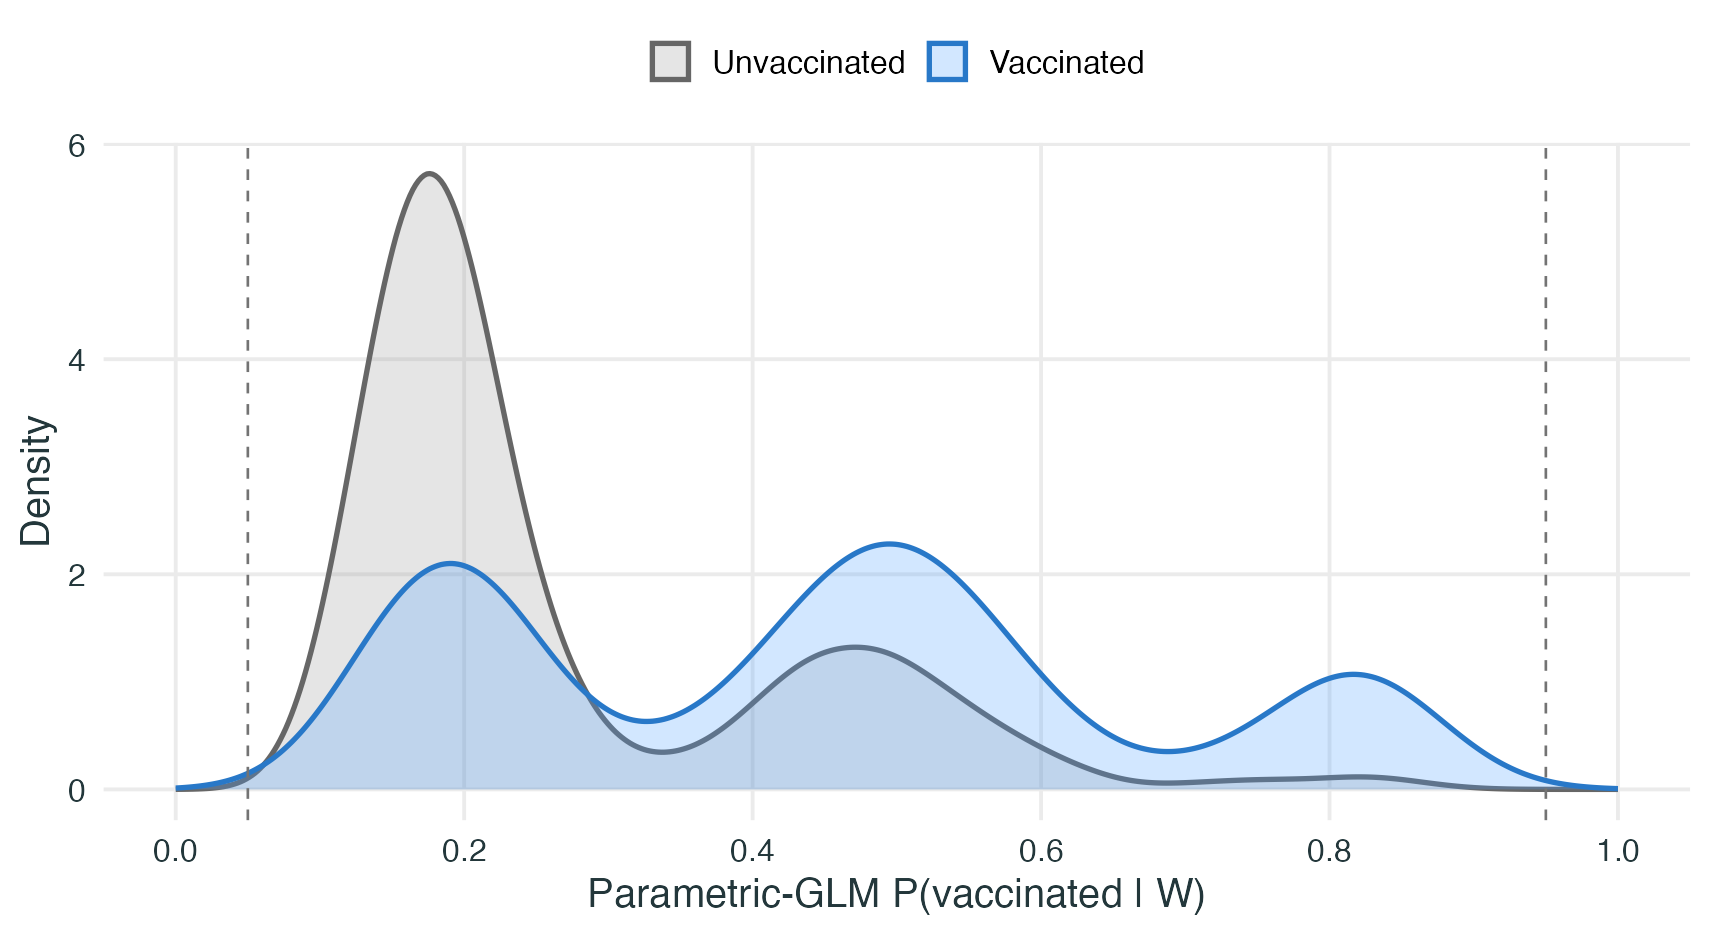
\includegraphics[width=\linewidth]{art/propensity_overlap.png}
    \end{column}
    \begin{column}{0.30\textwidth}
      \small
      \begin{block}{Parametric diagnostic}
        Range:
        \[
          0.077\text{ to }0.909
        \]
        Share outside \([0.05,0.95]\):
        \[
          0\%.
        \]
      \end{block}

      The plot assesses empirical support across measured \(W\); it does not
      test exchangeability.
    \end{column}
  \end{columns}
  \slidesource{Figure generated by
    \sourcefile{pneumonia_tmle_technical.R}; positivity guidance follows
    Petersen et al. (2012).}
\end{frame}

\begin{frame}{The Clever Covariate Focuses the Update}
  \small
  For a binary treatment and the average risk difference,
  \[
    H(A,W)
      =
    \frac{A}{\widehat g(W)}
      -
    \frac{1-A}{1-\widehat g(W)}.
  \]

  \vspace{0.45cm}
  Under the two intervention values:
  \[
    H(1,W)=\frac{1}{\widehat g(W)},
    \qquad
    H(0,W)=-\frac{1}{1-\widehat g(W)}.
  \]

  \vspace{0.55cm}
  Observations receiving a treatment that was less probable given \(W\)
  contribute more strongly to the targeted residual correction.
  \slidesource{Clever-covariate formula follows van der Laan and Rose (2011);
    implementation in \sourcefile{pneumonia_tmle_technical.R}.}
\end{frame}

\begin{frame}{A Logistic Fluctuation Estimates One Targeting Coefficient}
  \small
  Fit the intercept-free fluctuation model
  \[
    \operatorname{logit}E(Y\mid A,W)
      =
    \operatorname{logit}\widehat Q(A,W)
      +
    \epsilon H(A,W),
  \]
  where \(\operatorname{logit}\widehat Q(A,W)\) is an offset.

  \vspace{0.55cm}
  In the manual decomposition:
  \[
    \widehat\epsilon=0.008503.
  \]

  \vspace{0.55cm}
  The update is low-dimensional and parameter-focused: the complex learning
  happened in the initial nuisance fits.
  \slidesource{Fluctuation model and estimate from
    \sourcefile{pneumonia_tmle_technical.R}; method follows van der Laan and
    Rose (2011).}
\end{frame}

\begin{frame}{The Targeting Step Updates Both Intervention Predictions}
  \small
  \[
    \widehat Q^*(1,W)
      =
    \operatorname{expit}
    \left[
      \operatorname{logit}\widehat Q(1,W)
      +\widehat\epsilon\frac{1}{\widehat g(W)}
    \right],
  \]
  \[
    \widehat Q^*(0,W)
      =
    \operatorname{expit}
    \left[
      \operatorname{logit}\widehat Q(0,W)
      -\widehat\epsilon\frac{1}{1-\widehat g(W)}
    \right].
  \]

  \vspace{0.45cm}
  Because the update is on the logit scale, all targeted predictions remain in
  the valid probability range.
  \slidesource{Targeting equations follow van der Laan and Rose (2011);
    implementation in \sourcefile{pneumonia_tmle_technical.R}.}
\end{frame}

\begin{frame}{The TMLE Is a Plug-In Contrast of Updated Risks}
  \small
  \[
    \widehat\Psi_{\mathrm{TMLE}}
      =
    \frac{1}{n}\sum_{i=1}^n
    \left\{
      \widehat Q^*(1,W_i)-\widehat Q^*(0,W_i)
    \right\}.
  \]

  \vspace{0.5cm}
  \begin{columns}[T]
    \begin{column}{0.47\textwidth}
      \begin{block}{Manual decomposition}
        \centering
        \(-3.00\) percentage points
      \end{block}
    \end{column}
    \begin{column}{0.47\textwidth}
      \begin{block}{\codeword{tmle()} implementation}
        \centering
        \(-3.05\) percentage points
      \end{block}
    \end{column}
  \end{columns}

  \vspace{0.45cm}
  Small differences reflect implementation details in nuisance fitting and
  targeting; both use the same data, adjustment set, and estimand.
  \slidesource{Estimates from
    \sourcefile{outputs/pneumonia_tmle_technical_results.csv}.}
\end{frame}

\begin{frame}{The Efficient Influence Function Supplies Uncertainty}
  \footnotesize
  For the average risk difference,
  \[
  \begin{aligned}
    D^*(O)
      ={}&
      H(A,W)\{Y-Q^*(A,W)\}\\
      &+Q^*(1,W)-Q^*(0,W)-\Psi.
  \end{aligned}
  \]

  \vspace{0.35cm}
  Estimate
  \[
    \widehat{\operatorname{SE}}(\widehat\Psi)
      =
    \frac{\operatorname{sd}\{\widehat D^*(O_i)\}}{\sqrt n},
    \qquad
    \widehat\Psi\pm1.96\,\widehat{\operatorname{SE}}.
  \]

  \vspace{0.45cm}
  The manual implementation has
  \(\overline{\widehat D^*}=-8.8\times10^{-13}\), a numerical check that the
  targeted estimating equation is solved. Its SE is \(0.802\) percentage
  points.
  \slidesource{EIF formula follows van der Laan and Rose (2011); diagnostics
    from \sourcefile{outputs/pneumonia_tmle_technical_diagnostics.csv}.}
\end{frame}

\begin{frame}[fragile]{Manual Step 1: Fit \(Q\) and \(g\)}
  \begin{lstlisting}[language=R]
learners <- c("SL.glm", "SL.glmnet", "SL.ranger")

Q_fit <- SuperLearner(
  Y = Y, X = data.frame(A = A, W),
  family = binomial(), SL.library = learners,
  cvControl = list(V = 3L)
)
QAW <- Q_fit$SL.predict
Q1  <- predict(Q_fit, data.frame(A = 1, W))$pred
Q0  <- predict(Q_fit, data.frame(A = 0, W))$pred

g_fit <- SuperLearner(
  Y = A, X = W, family = binomial(),
  SL.library = learners, cvControl = list(V = 3L)
)
g <- pmin(pmax(g_fit$SL.predict, 0.025), 0.975)
H <- A / g - (1 - A) / (1 - g)
  \end{lstlisting}
  \slidesource{Abbreviated from
    \sourcefile{pneumonia_tmle_technical.R}; SuperLearner API version 2.0-29.}
\end{frame}

\begin{frame}[fragile]{Manual Step 2: Target, Average, and Form the Interval}
  \begin{lstlisting}[language=R]
fluctuation <- glm(
  Y ~ -1 + H + offset(qlogis(QAW)),
  family = binomial()
)
epsilon <- coef(fluctuation)[["H"]]

Q1_star <- plogis(qlogis(Q1) + epsilon / g)
Q0_star <- plogis(qlogis(Q0) - epsilon / (1 - g))
QAW_star <- plogis(qlogis(QAW) + epsilon * H)

psi <- mean(Q1_star - Q0_star)
eif <- H * (Y - QAW_star) +
  Q1_star - Q0_star - psi
se <- sd(eif) / sqrt(length(Y))
ci <- psi + qnorm(c(0.025, 0.975)) * se
  \end{lstlisting}
  \slidesource{Abbreviated from
    \sourcefile{pneumonia_tmle_technical.R}; targeting formula follows van der
    Laan and Rose (2011).}
\end{frame}

\begin{frame}[fragile]{The Package Implementation Encapsulates the Same Sequence}
  \begin{lstlisting}[language=R]
fit <- tmle(
  Y = Y, A = A, W = W,
  Q.SL.library = learners,
  g.SL.library = learners,
  V.Q = 3, V.g = 3
)

psi <- fit$estimates$ATE$psi
ci  <- fit$estimates$ATE$CI

g1W <- fit$g$g1W
Q0_initial <- fit$Qinit$Q[, "Q0W"]
Q1_initial <- fit$Qinit$Q[, "Q1W"]
Q0_updated <- fit$Qstar[, "Q0W"]
Q1_updated <- fit$Qstar[, "Q1W"]
  \end{lstlisting}

  \footnotesize
  The manual version exposes the mechanics; the package version is the
  practical analysis route.
  \slidesource{Verified object fields for tmle 2.1.1; executable call in
    \sourcefile{pneumonia_tmle_technical.R}.}
\end{frame}

\begin{frame}{The Technical Results Keep Every Estimator on One Scale}
  \small
  \centering
  \begin{tabular}{@{}lrrr@{}}
    \toprule
    \textbf{Estimator} & \textbf{RD (pp)} & \textbf{95\% lower} &
      \textbf{95\% upper} \\
    \midrule
    Crude association & \(+0.76\) & -- & -- \\
    Parametric g-computation & \(-3.28\) & -- & -- \\
    Hajek IPW & \(-2.94\) & -- & -- \\
    Manual TMLE decomposition & \(-3.00\) & \(-4.57\) & \(-1.43\) \\
    \codeword{tmle()} package & \(-3.05\) & \(-4.60\) & \(-1.50\) \\
    \midrule
    DGP benchmark (frozen \(W\)) & \(-4.04\) & -- & -- \\
    \bottomrule
  \end{tabular}

  \vspace{0.65cm}
  The benchmark averages model-implied counterfactual risks over the frozen
  covariate distribution; it would not be observed in an applied analysis.
  \slidesource{Results from
    \sourcefile{outputs/pneumonia_tmle_technical_results.csv}; benchmark from
    \sourcefile{simulate_pneumonia_data.R}.}
\end{frame}

\begin{frame}{The Estimator Comparison Separates Association from Adjustment}
  \centering
  \vspace{-0.2cm}
  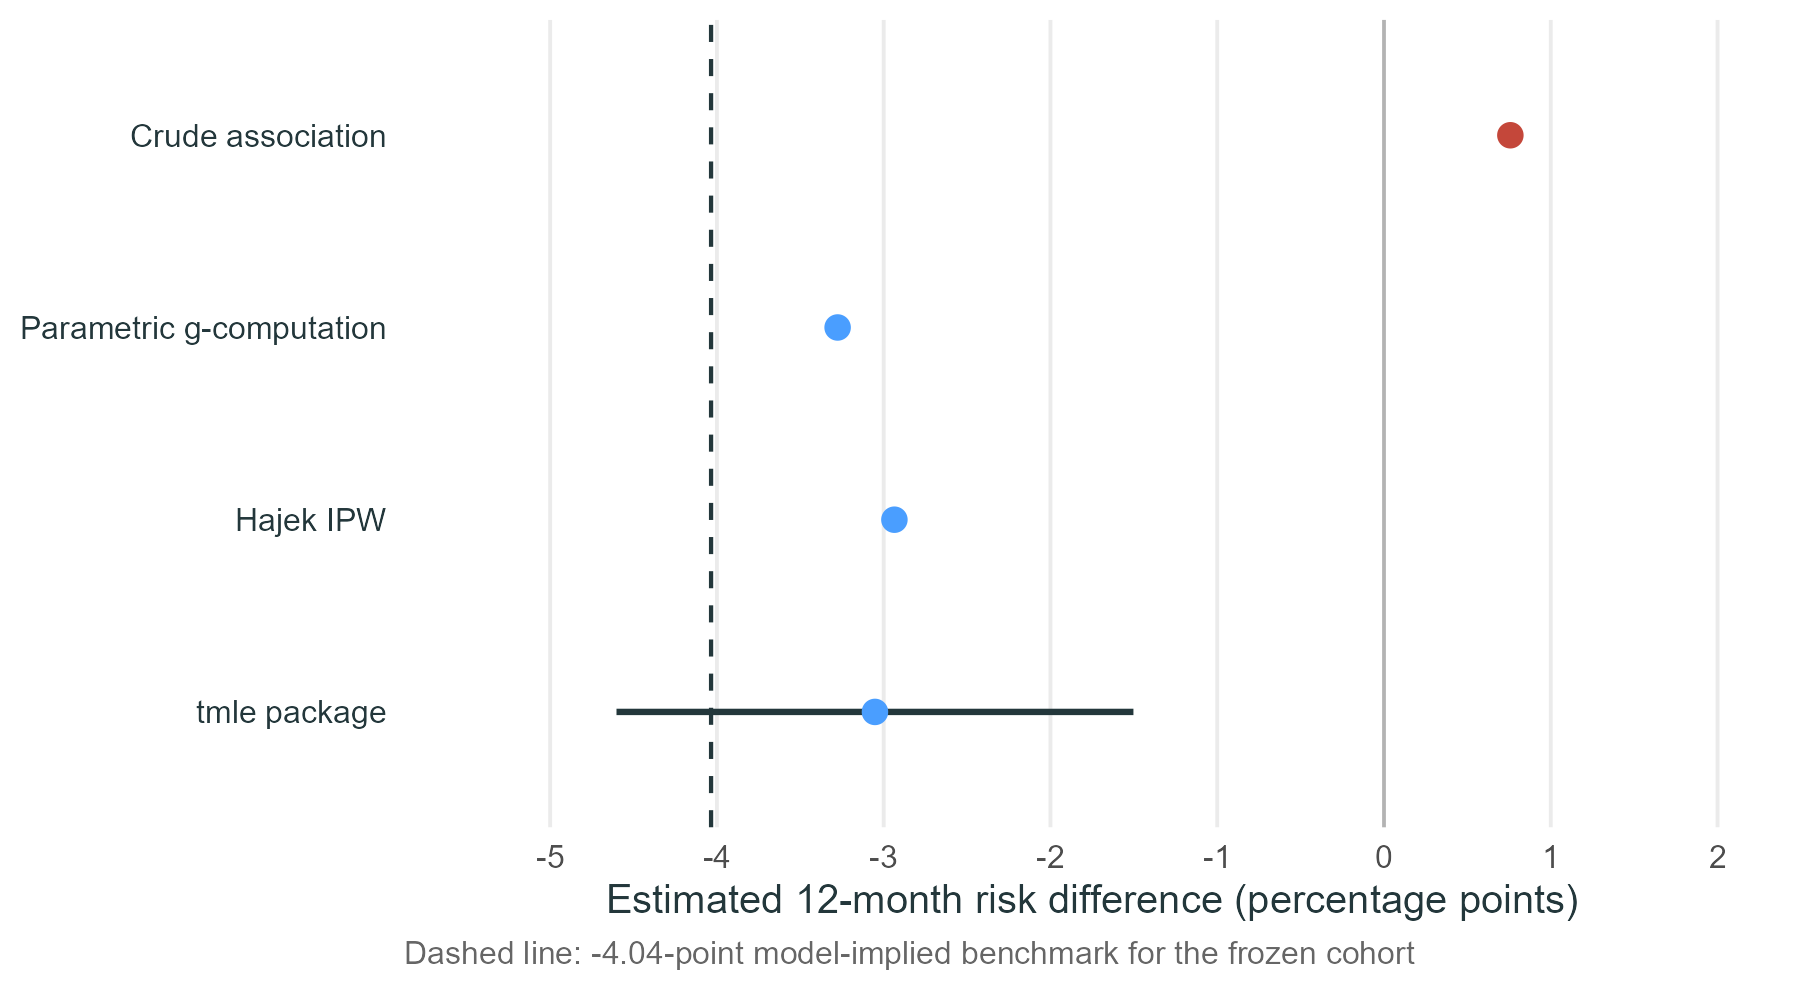
\includegraphics[width=0.82\textwidth]{art/estimator_comparison.png}

  \vspace{-0.1cm}
  \footnotesize
  The adjusted estimators recover a protective direction in this sample. Their
  similarity is useful for implementation review, while causal validity still
  depends on the shared study assumptions.
  \slidesource{Figure generated by
    \sourcefile{pneumonia_tmle_technical.R}.}
\end{frame}

\begin{frame}{Double Robustness Uses Information from Both Nuisance Models}
  \small
  For a point-treatment average effect, TMLE is consistent under appropriate
  regularity and positivity conditions if either
  \[
    \widehat Q \longrightarrow Q_0
    \qquad\text{or}\qquad
    \widehat g \longrightarrow g_0.
  \]

  \vspace{0.55cm}
  \begin{columns}[T]
    \begin{column}{0.47\textwidth}
      \textbf{Practical implication}
      \begin{itemize}
        \item Fit both nuisance functions carefully.
        \item Inspect support and prediction behavior.
        \item Use flexible learners when justified.
      \end{itemize}
    \end{column}
    \begin{column}{0.47\textwidth}
      \textbf{Scope}
      \begin{itemize}
        \item This is an estimator property.
        \item It does not identify unmeasured confounding.
        \item Finite-sample performance can still be poor.
      \end{itemize}
    \end{column}
  \end{columns}
  \slidesource{Double-robustness result follows van der Laan and Rose (2011)
    and Kennedy (2023).}
\end{frame}

\begin{frame}{Positivity Diagnostics Guide the Estimand and Analysis Population}
  \small
  When \(\widehat g(W)\) approaches 0 or 1,
  \[
    \left|H(A,W)\right|
  \]
  can become large, increasing variance and sensitivity to nuisance-model
  error.

  \vspace{0.45cm}
  \begin{columns}[T]
    \begin{column}{0.47\textwidth}
      \textbf{Analysis options}
      \begin{itemize}
        \item Improve design or data collection
        \item Restrict to a population with shared support
        \item Use a treatment rule or overlap-weighted target
      \end{itemize}
    \end{column}
    \begin{column}{0.47\textwidth}
      \textbf{Truncation}
      \begin{itemize}
        \item Can stabilize an estimator
        \item Introduces a bias-variance tradeoff
        \item Should be prespecified and sensitivity-analyzed
      \end{itemize}
    \end{column}
  \end{columns}
  \slidesource{Positivity and truncation discussion follows Petersen et al.
    (2012) and van der Laan and Rose (2011).}
\end{frame}

\begin{frame}{Influence-Curve Inference Requires Rate and Regularity Conditions}
  \small
  The usual Wald interval relies on an asymptotic linear expansion:
  \[
    \widehat\Psi-\Psi_0
      =
    \frac{1}{n}\sum_{i=1}^n D^*(O_i)
      +o_p(n^{-1/2}).
  \]

  \vspace{0.4cm}
  A key remainder is controlled when the product of nuisance errors is small:
  \[
    \|\widehat Q-Q_0\|\,\|\widehat g-g_0\|
      =o_p(n^{-1/2}).
  \]

  \vspace{0.5cm}
  Cross-fitting can reduce empirical-process restrictions for highly adaptive
  learners. The workshop script uses the standard single-fit \codeword{tmle}
  implementation with cross-validated Super Learner nuisance fits.
  \slidesource{Rate-condition and cross-fitting discussion follows Chernozhukov
    et al. (2018) and Kennedy (2023).}
\end{frame}

\begin{frame}{The Causal Interpretation Retains the Navigator Assumptions}
  \small
  \begin{columns}[T]
    \begin{column}{0.47\textwidth}
      \textbf{Identification}
      \begin{itemize}
        \item Exchangeability given measured \(W\)
        \item Positivity in the target population
        \item Consistency of treatment versions
      \end{itemize}

      \vspace{0.3em}
      \textbf{Measurement}
      \begin{itemize}
        \item Correct vaccination classification
        \item Correct hospitalization ascertainment
      \end{itemize}
    \end{column}
    \begin{column}{0.47\textwidth}
      \textbf{Time and selection}
      \begin{itemize}
        \item Common eligibility and treatment time zero
        \item Complete or appropriately modeled follow-up
        \item Appropriate handling of missingness and selection
      \end{itemize}

      \vspace{0.3em}
      \textbf{Transport}
      \begin{itemize}
        \item The target population is the synthetic cohort
        \item No clinical generalization is intended
      \end{itemize}
    \end{column}
  \end{columns}
  \slidesource{Assumption set follows the Navigator roadmap and Hernan and
    Robins (2020).}
\end{frame}

\begin{frame}{The Audit Trail Connects Data, Code, Output, and Session State}
  \scriptsize
  \begin{tabular}{@{}p{0.32\textwidth}p{0.58\textwidth}@{}}
    \toprule
    \textbf{Artifact} & \textbf{Role} \\
    \midrule
    \sourcefile{data/pneumonia_data.csv} &
      Frozen cohort used throughout the Navigator and Segment G \\
    \sourcefile{simulate_pneumonia_data.R} &
      Structural equations, legacy-state reproduction, and value check \\
    \sourcefile{pneumonia_tmle_example.R} &
      Short live analysis \\
    \sourcefile{pneumonia_tmle_technical.R} &
      Manual decomposition, package fit, diagnostics, plots, and outputs \\
    \sourcefile{outputs/*.csv} &
      Machine-readable estimates and diagnostics \\
    \sourcefile{outputs/session_info.txt} &
      R and package environment \\
    \bottomrule
  \end{tabular}

  \vspace{0.6cm}
  Rebuilding begins with the technical R script, then compiles each Beamer
  source twice.
  \slidesource{Artifact roles and build order from the Segment G package.}
\end{frame}

\begin{frame}{TMLE, AIPW, and DML Share an Orthogonal-Score Perspective}
  \scriptsize
  \begin{tabular}{@{}p{0.18\textwidth}p{0.24\textwidth}p{0.24\textwidth}p{0.22\textwidth}@{}}
    \toprule
    & \textbf{TMLE} & \textbf{AIPW / one-step} & \textbf{DML} \\
    \midrule
    Core idea &
      Target an initial plug-in fit &
      Add an influence-function correction &
      Estimate an orthogonal score with sample splitting \\
    Nuisance functions &
      \(Q\) and \(g\) &
      \(Q\) and \(g\) &
      Problem-specific nuisance functions \\
    Parameter space &
      Plug-in estimate respects outcome bounds &
      One-step estimate need not be substitution-based &
      Depends on score and target \\
    Inference &
      EIF-based under regularity/rate conditions &
      EIF-based under regularity/rate conditions &
      Orthogonal-score inference, typically cross-fitted \\
    \bottomrule
  \end{tabular}

  \vspace{0.45cm}
  These are related frameworks, not interchangeable labels; implementation
  details and target parameters determine the exact guarantees.
  \slidesource{Comparison follows van der Laan and Rose (2011), Chernozhukov
    et al. (2018), and Kennedy (2023).}
\end{frame}

\begin{frame}{Technical Takeaways}
  \small
  \begin{enumerate}
    \item The Navigator fixes the population, time order, adjustment set, and
      risk-difference target before estimation.
    \item TMLE begins with flexible estimates of \(Q(A,W)\) and \(g(W)\).
    \item The clever covariate and logistic fluctuation target \(Q\) for the
      selected parameter.
    \item Averaging \(Q^*(1,W)-Q^*(0,W)\) gives a substitution estimate.
    \item The efficient influence function supports the standard error and
      provides an estimating-equation diagnostic.
    \item Double robustness and machine learning improve estimation under
      stated conditions; the causal interpretation retains the study
      assumptions.
  \end{enumerate}

  \vspace{0.45cm}
  \begin{block}{Reproducible result}
    \(\widehat\Psi_{\mathrm{TMLE}}=-3.05\) percentage points,
    95\% CI \([-4.60,-1.50]\), in synthetic teaching data.
  \end{block}
  \slidesource{Summary of the Segment G technical workflow and verified
    outputs.}
\end{frame}

\begin{frame}{References: Causal Inference and Targeted Learning}
  \scriptsize
  \begin{thebibliography}{99}
    \bibitem{hernan2020}
      Hernan MA, Robins JM. \emph{Causal Inference: What If}. Chapman \&
      Hall/CRC; 2020.
    \bibitem{petersen2012}
      Petersen ML, Porter KE, Gruber S, Wang Y, van der Laan MJ. Diagnosing and
      responding to violations in the positivity assumption.
      \emph{Statistical Methods in Medical Research}. 2012.
    \bibitem{petersen2014}
      Petersen ML, van der Laan MJ. Causal models and learning from data:
      integrating causal modeling and statistical estimation.
      \emph{Epidemiology}. 2014.
    \bibitem{tl2011}
      van der Laan MJ, Rose S. \emph{Targeted Learning}. Springer; 2011.
  \end{thebibliography}
  \slidesource{Full bibliographic entries shown on slide.}
\end{frame}

\begin{frame}{References: Machine Learning and Inference}
  \tiny
  \begin{thebibliography}{99}
    \bibitem{chernozhukov2018}
      Chernozhukov V, et al. Double/debiased machine learning for treatment
      and structural parameters. \emph{The Econometrics Journal}. 2018.
    \bibitem{kennedy2023}
      Kennedy EH. Semiparametric doubly robust targeted double machine
      learning: a review. \emph{arXiv:2203.06469}. 2023.
    \bibitem{sl2007}
      van der Laan MJ, Polley EC, Hubbard AE. Super Learner.
      \emph{Statistical Applications in Genetics and Molecular Biology}. 2007.
  \end{thebibliography}
  \slidesource{Full bibliographic entries shown on slide; software versions in
    \sourcefile{outputs/session_info.txt}.}
\end{frame}

\end{document}
